
Electric dipole moments  are the P- and CP-odd  
counterparts (from CPT conservation) to magnetic moments. They arise from a set of  ${O}^{(6)}_{a}$ operators in Eq.~(\ref{effective}) which flip the chirality of a fermion  and involve the EW field strengths and the Higgs doublet. After spontaneous symmetry breaking they result in a coupling 
of the fermion spin $\vec{\sigma}$ to the electric field $\vec{E}$ of the form $d\,\vec{\sigma} \cdot \vec{E}$, where $d$  denotes the  EDM strength.

\begin{figure}
\begin{center}
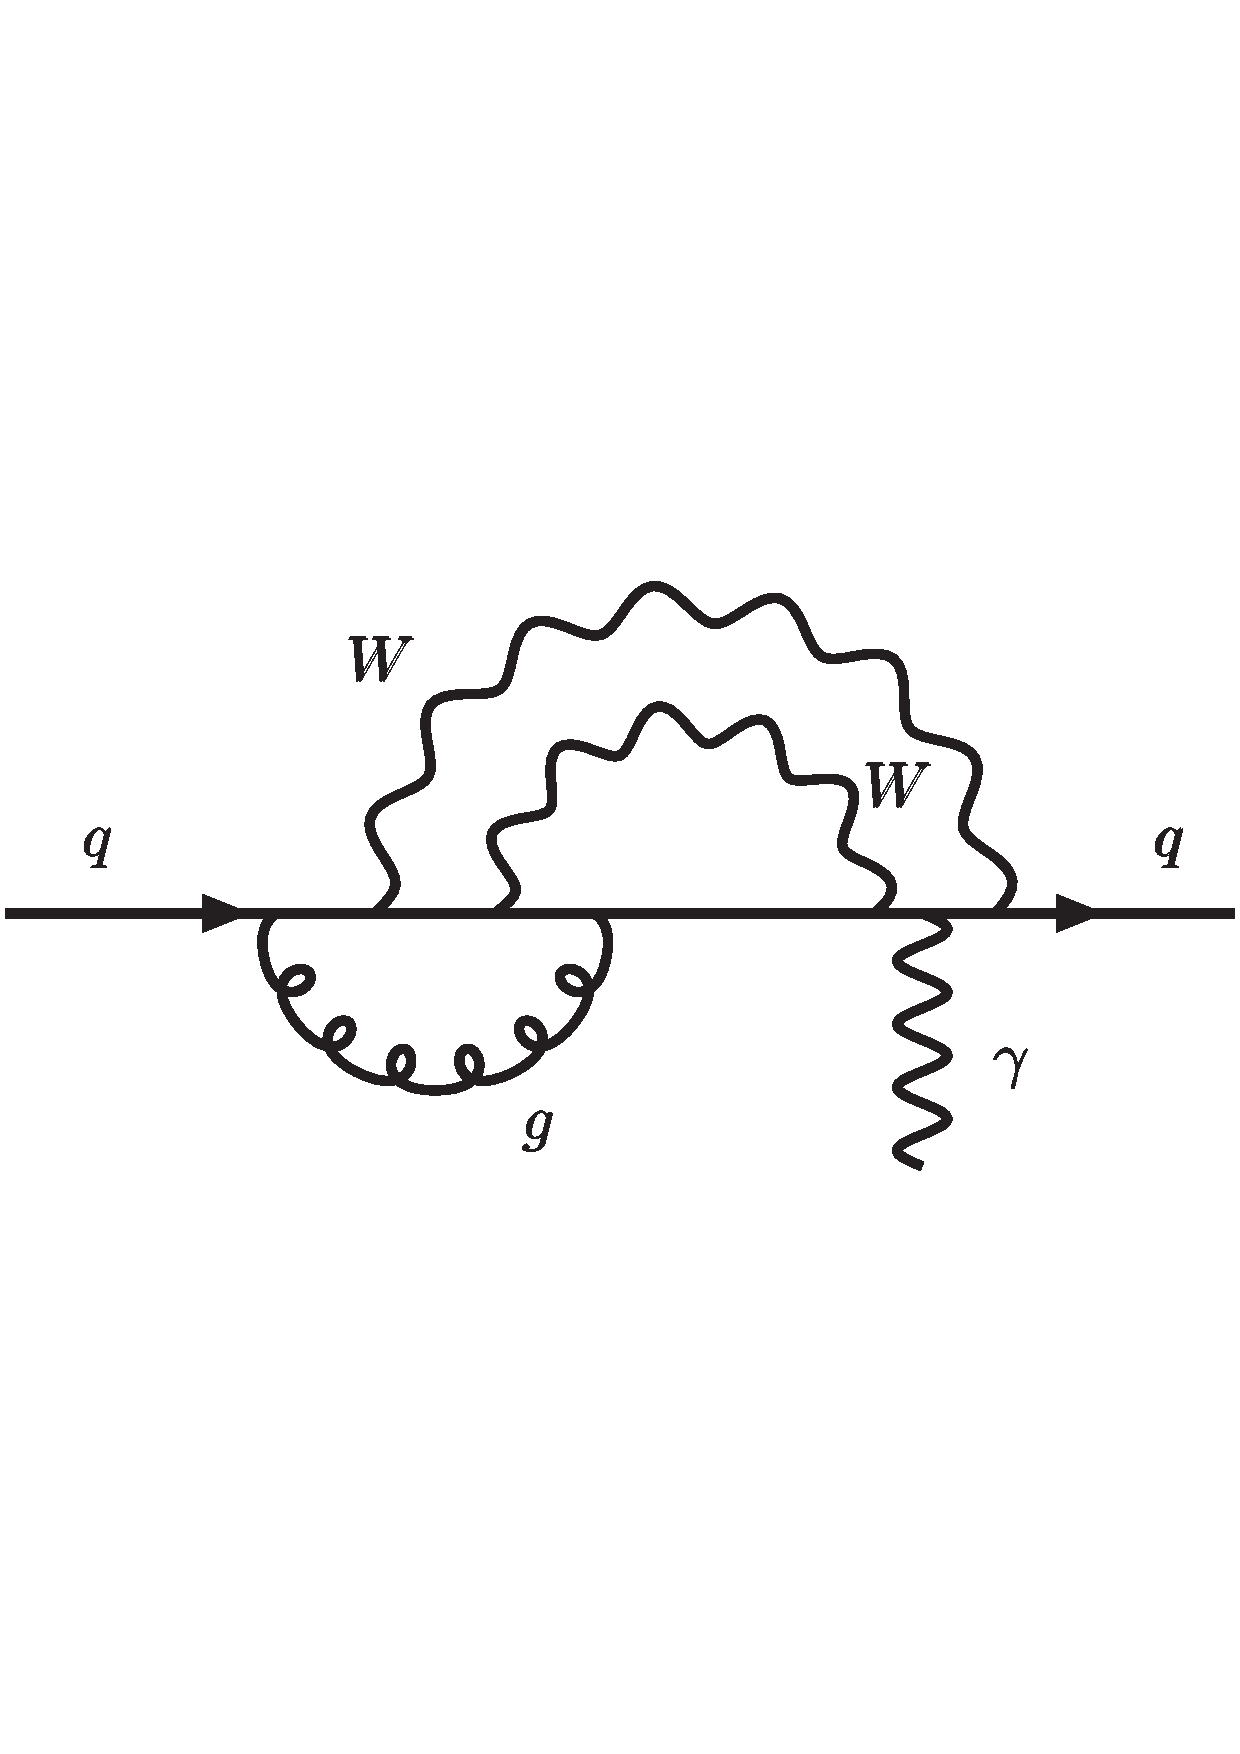
\includegraphics[width=0.43\textwidth]{\main/Flavour/figs/EDM_SM} \hspace*{5mm}
\raisebox{10mm}{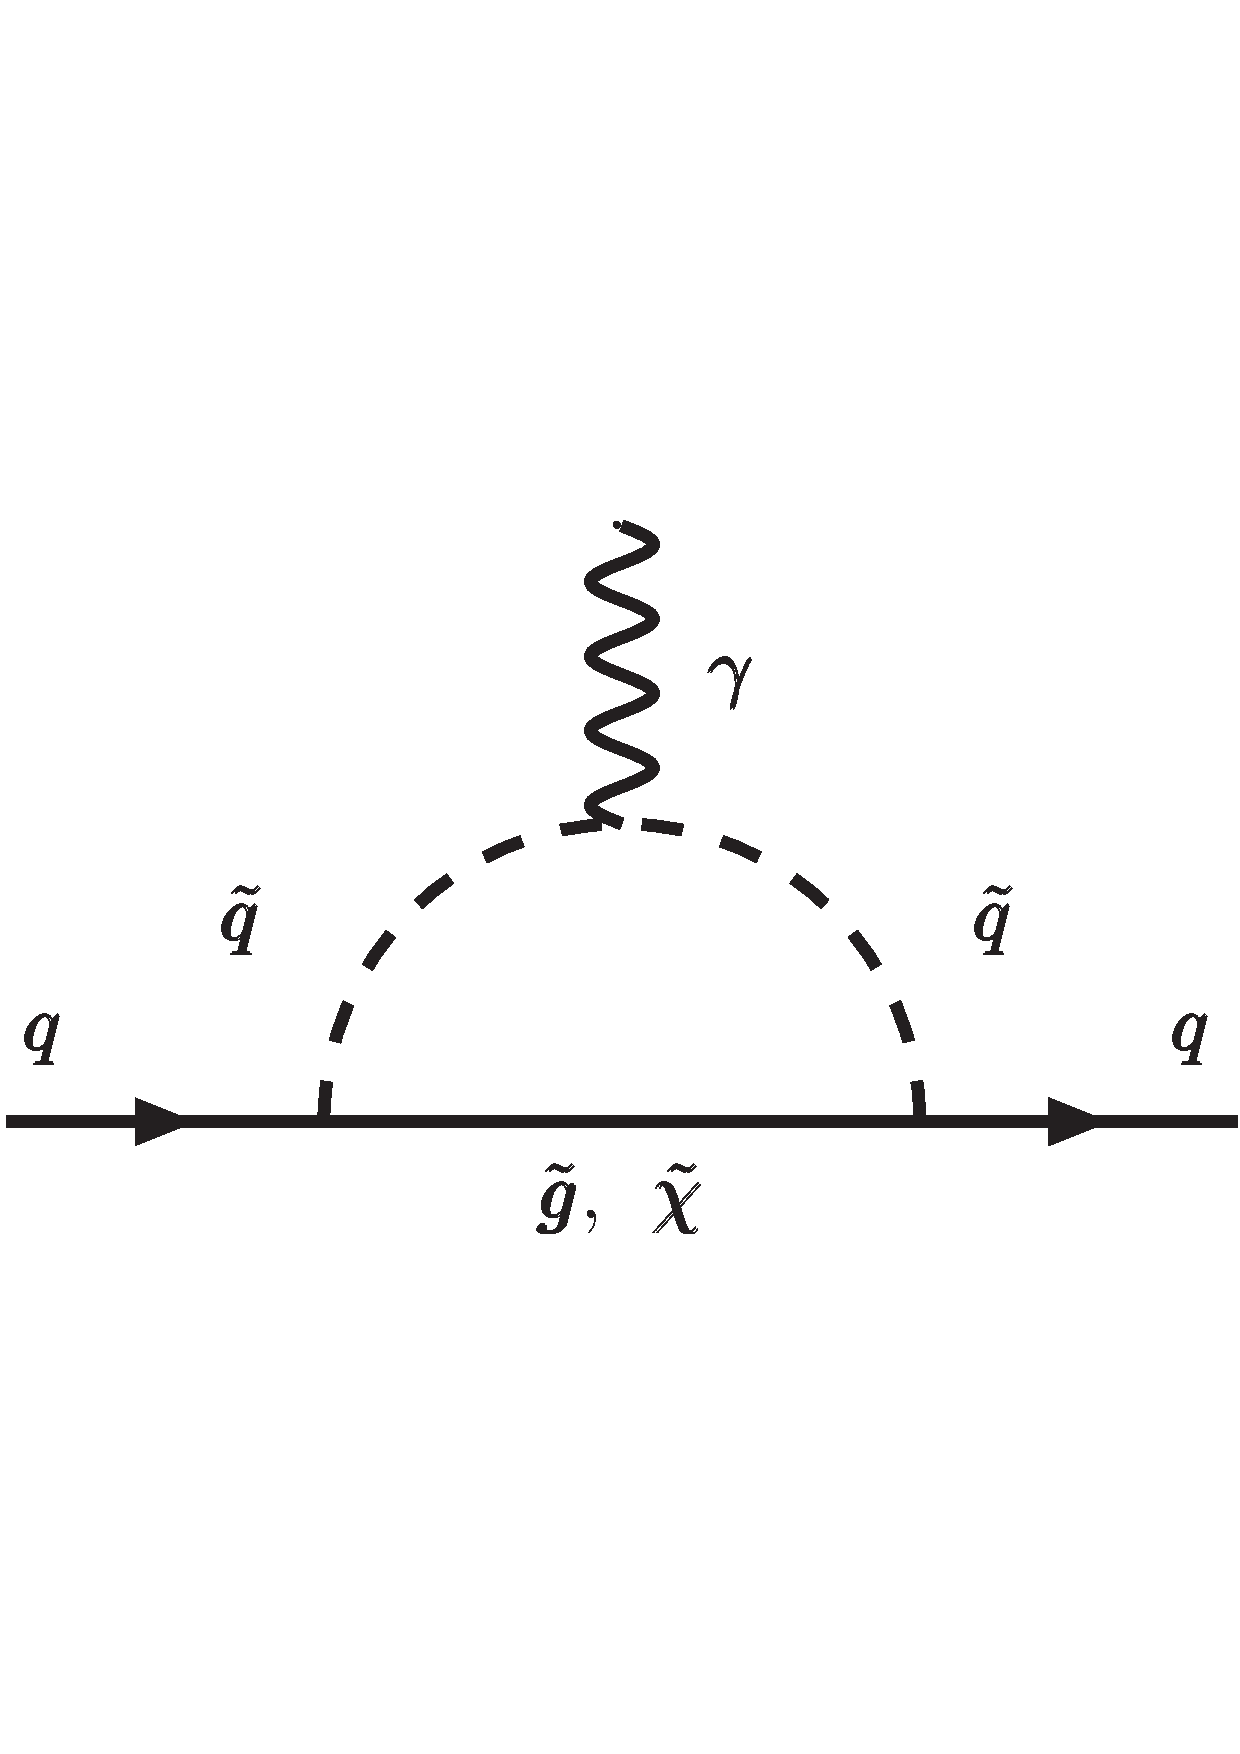
\includegraphics[width=0.37\textwidth]{\main/Flavour/figs/EDM_SUSY} }
\end{center}
\caption{On the left, one example of SM contribution to the quark EDM; on the right, one-loop new physics contribution, exemplified by a generic supersymmetric  contribution mediated by squarks and gauginos. }\label{fig:FeynEDM} 
\end{figure}

The EDMs are clean and powerful probes of new physics (NP).  
In the SM, the
EW contributions to quark EDMs arise only at 3 loop-level and are
extremely suppressed due to the chiral nature of the SM flavour changing currents: the predictions lie well below present sensitivities. The same applies to leptons taking into account the known structure of neutrino masses and mixings. 
In contrast, most new physics models   
include new mediators and  new sources of CP violation that can generate  EDMs already at one-loop level, see Fig.~\ref{fig:FeynEDM}. The bounds on the EDMs thus severely constrain NP scenarios. For instance, 
in the absence of a suppression mechanism the new contributions to the EDMs can be easily in 
the range of $10^{-23}- 10^{-25}$~e$\cdot$cm, which is already in conflict with the present experimental bounds. Note that the EDMs are null searches; any nonzero signal at present or projected sensitivities would imply new physics.


The quark (or hadron) EDM and lepton EDM searches are complementary, as they may test different physics.  The leptonic  EDM is necessarily sourced by EW physics, while the hadronic EDMs are sensitive to both the EW and the strong interactions, for instance the $\theta$  parameter of QCD. 
The EDM searches are also
complementary to the high-energy CP probes, since they probe a different combination of NP parameters. 
 The combination of
quark and lepton searches for CP violation at different frontiers is
thus a formidable tool to test for NP. 



